\chapter{Test Cases}
\label{chap:landice_test_cases}

Eventually test case will be available for download.  Currently they are only part of the Development code for MPAS-Land Ice.

%%%All test cases can be downloaded from \url{http://mpas-dev.github.com}  The test cases for this version of the code are available at\\
%%%\url{http://mpas-dev.github.com/ocean/release_\version/release_\version.}.

\FloatBarrier


\section{Halfar Dome}
\label{sec:halfar_description}
This test case describes the time evolution of a dome of ice as described by \citet{Halfar1983}.
This test provide an analytic solution for a flat-bedded SIA problem.

\begin{equation}
    \label{halfar}
    \frac{\partial H}{\partial t} = \nabla \cdot (\Gamma H^{n+2} |\nabla H|^{n-1} \nabla H)
\end{equation}
where $n$ is the exponent in the Glen flow law, commonly taken as 3, and $\Gamma$ is a positive constant:
\begin{equation}
    \Gamma = \frac{2}{n+2} A (\rho g)^n
\end{equation}

For $n=3$, this reduces to:
\begin{equation}
    H(t,r) = H_0 \left(\frac{t_0}{t}\right)^\frac{1}{9}  \left[ 1 - \left(  \left( \frac{t_0}{t} \right) ^ \frac{1}{18} \frac{r}{R_0} \right)^\frac{4}{3} \right] ^ \frac{3}{7}
\end{equation}
where
\begin{equation}
    t_0 = \frac{1}{18\Gamma} \left( \frac{7}{4} \right)^3 \frac{R_0^4}{H_0^7}
\end{equation}
and $H_0, R_0$ are the central height of the dome and its radius at time $t=t_0$.

For more details see \url{http://www.projects.science.uu.nl/iceclimate/karthaus/2009/more/lecturenotes/EdBueler.pdf},  \citet{Bueler2005}, \citet{Halfar1983}.



\subsection{Provided Files}
\label{subsec:halfar_files}
Our implementation of the Halfar dome has an initial radius of $R_0=21.2$ km and an initial thickness of $H=707.1$ m.
These values can be changed by editing \texttt{setup\_dome\_initial\_conditions.py}.

\begin{itemize}
	\item readme.txt: \\
		Information about the test case.
	\item namelist.input.periodic\_hex: \\
		This is the namelist file to use for creating the grid file for the run. \\
		It is used with the \texttt{periodic\_hex} grid generator.  \\
		It should be renamed to \texttt{namelist.config} when executing \texttt{periodic\_hex}. \\
		periodic\_hex will be used to generate \texttt{grid.nc} which can be used to create \\
		\texttt{landice\_grid.nc} and \texttt{graph.info.part.*} which can be used for running the model \\
		on more than one processor.
	\item setup\_dome\_initial\_conditions.py: \\
		This python script generates the dome initial condition after \\
		an empty \texttt{landice\_grid.nc} file exists.
	\item namelist.input.landice\_core: \\
		This is the namelist file to use for running the model with \texttt{landice\_model}. \\
		It should be renamed to \texttt{namelist.config} when executing \texttt{landice\_model}.
	\item halfar.py: \\
		This is the script to compare model results to the analytic solution.
	\item visualize\_dome.py: \\
		This python script provides some general visualization of the model output.
		It can be used in addition to \texttt{halfar.py} for additional visualization.
\end{itemize}

\subsection{Results}
\label{subsecc:halfar_results}
As the dome of ice evolves, its margin advances and its thickness decreases (there is no surface mass balance to add new mass).  The script \texttt{halfar.py} will plot the modeled and analytic thickness at a specified time (Figure \ref{fig:halfarresults}), as well as report model error statistics.  Invoke \texttt{halfar.py --help} for details of its usage.


\begin{figure}[H!]
	\centering
	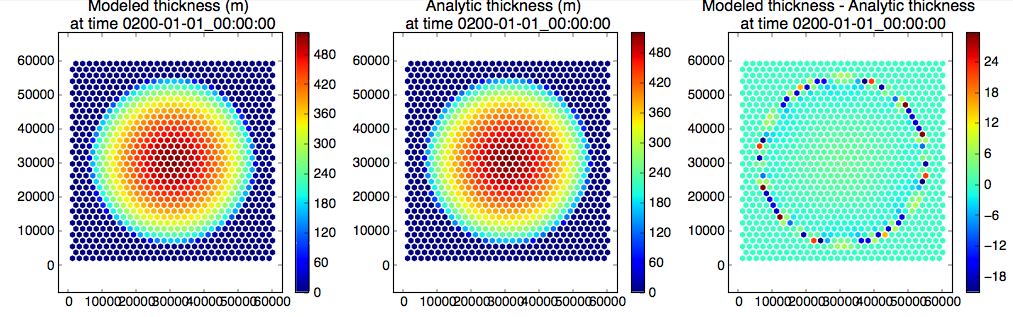
\includegraphics[width=16.4cm]{landice/figures/halfar.png}
	\caption{Halfar test case results after 200 years of dome evolution. This figure is generated by \texttt{halfar.py}.}
	\label{fig:halfarresults}
\end{figure}


\FloatBarrier


\section{Real World Test Cases}
Eventually grids for real-world Greenland and Antarctica will be provided at varying resolutions.


